\chapter{Jet smearing method}
    \label{app:JetSmearingMethod}

The large $\met$ in the multijet background originates mainly from the misreconstruction of the energy of the jets in the calorimeter, and to a lesser extent, due to the presence of neutrinos in the decays of heavy flavor hadrons.
The multijet processes represent a small contribution to the total background in the selection M1, and are almost negligible in the other selections.

The method to estimate the multijet processes relies on the assumption that the $\met$ of these events has its origin in the fluctuations in the response of the calorimeter.
This method, also known as the \emph{jet smearing method}, proceeds in four steps, detailed in the following:    

\begin{enumerate}
\item{\textbf{Seed sample}} A sample of multijet events is selected with a lower cut on the leading jet $\pt$ of 100~GeV.
In order to select well-balanced events, a cut on the significance of the missing transverse energy,
\begin{equation}
\met / \sqrt{\sum{\et}} < 1.0,
\label{eq:JetSmearingMetSignificance}
\end{equation}

\noindent is required.
This seed sample is then used in steps 3 and 4.

\item{\textbf{Response function}}  Two jet \emph{response functions}, one for jets with b-veto and another for $b$-tagged jets\footnote{The MV1 $b$-tagger is used.}, are extracted from the simulation to estimate the fluctuations in the measured jet transverse momenta and the contributions from neutrinos from heavy flavor decays.
They are estimated by comparing the generator level to reconstructed jet transverse momenta distribution.
This is the only part where the MC simulation is used.
The two response functions are shown in Figure~\ref{fig:JetSmearingResponseFunctions}.

\begin{figure}[!ht]
  \begin{center}
    \mbox{
      \includegraphics[width=0.495\textwidth]{Appendix_JetSmearingMethod/Figures/jetsmearing25_R_btag.eps}
      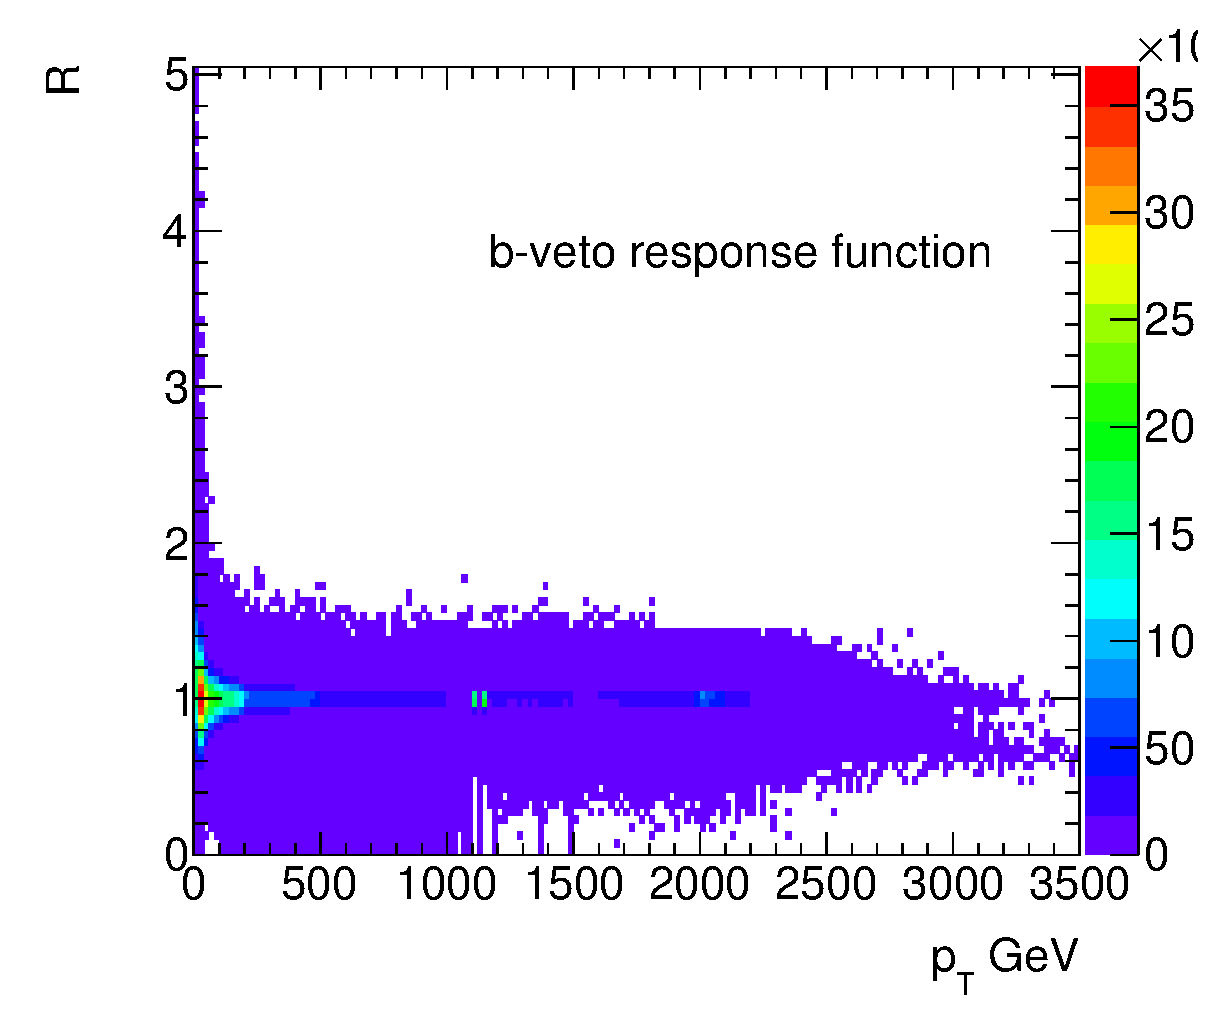
\includegraphics[width=0.495\textwidth]{Appendix_JetSmearingMethod/Figures/jetsmearing25_R_bveto.eps}
    }
  \end{center}
  \caption{Response functions for $b$-tag jets and $b$-veto jets}
  \label{fig:JetSmearingResponseFunctions}
\end{figure}

\item{\textbf{Adjusted response function}} The response function from step 2 is used to smear the seed events from step 1.
In the analysis, a total of 500 smeared events are produced from each seed event.
Further corrections as a function of the $\phi$-direction of the jet are also applied to the smeared jets.

\item{\textbf{Extrapolation to SR}} The seed events from step 1 are now smeared with the adjusted response function from step 3 to estimate the distributions of relevant variables in the control and signal regions.
After the seed events are smeared, the multijet contribution needs to be normalized in a dedicated control region.
The multijet control regions are defined with exactly the same cuts as the different signal regions M1-M6 (see Table \ref{tab:SignalRegionCuts}), but reverting the $\Delta\phi(\text{jet}, \mathbf{p_{T}}^\text{miss})$ cut to be below 0.4.
The contribution from the other backgrounds ($W/Z$+jets, single top and $\ttbar$, dibosons) are subtracted using MC simulations, normalized with the normalization factors from the global fit (see Section~\ref{sec:Fit}), when appropriate.
As an example, the relevant distributions of the smeared events for the region M1 are shown in Figure \ref{fig:JetSmearingCheckPlots}.

\end{enumerate}

The normalization factors and the estimation of the multijet background for the signal regions M1 to M6 are shown in Table~\ref{tab:qcd_est}.
This table also shows the fraction of multijet events in the total background prediction.

Finally, in order to determine the systematic uncertainty on the multijet prediction, the multijet yields calculated with different response functions, are compared.
Variations in the multijet yield of the order of 100\% have been observed.
For this reason, a 100\% systematic uncertainty is assigned to the estimated number of events.

%--- \ref{tab:qcd_est}
\begin{sidewaystable}[!htb]
\begin{center}
\vspace*{1em}
\begin{tabular}{ccccc}
\hline\hline
\multicolumn{5}{c}{\textbf{Multijet Estimation}} \\
\hline
\multirow{2}{*}{\textbf{SR}}  & \textbf{Normalization} & \multirow{2}{*}{\textbf{Estimation}}    & \multirow{2}{*}{\textbf{stat. $\pm$ sys. uncert.}} & \textbf{Total background}  \\
                              & \textbf{factor}        &                                         &                                   & \textbf{fraction} \\
\hline
M1  & 0.005 & \phantom{1}315.4 $\pm$           17.8 $\pm$ 315.4 &    ($\pm$ \phantom{11}6 $\pm$ 100)\%   & 0.9\%   \\
M2  & 0.006 & \phantom{11}29.7 $\pm$ \phantom{1}5.5 $\pm$ 29.7 &    ($\pm$ \phantom{1}18 $\pm$ 100)\%   & 0.3\%   \\
M3  & 0.006 & \phantom{111}3.6 $\pm$ \phantom{1}1.9 $\pm$ 3.6 &    ($\pm$ \phantom{1}53 $\pm$ 100)\%   & 0.1\%    \\
M4  & 0.005 & \phantom{111}6.8 $\pm$ \phantom{1}2.6 $\pm$ 6.8 &    ($\pm$ \phantom{1}38 $\pm$ 100)\%   & 0.3\%    \\
M5  & 0.006 & \phantom{111}0.7 $\pm$ \phantom{1}0.8 $\pm$ 0.6 &    ($\pm$           120 $\pm$ 100)\%   & 0.1\%    \\
M6  & 0.006 & \phantom{111}0.4 $\pm$ \phantom{1}0.7 $\pm$ 0.4 &    ($\pm$           150 $\pm$ 100)\%   & 0.1\%    \\
\hline\hline
\end{tabular}
\end{center}
\caption[Normalizations and final estimates of the multijet contribution for the signal regions M1 to M6.]
{Normalizations and final estimates of the multijet contribution for the signal regions M1 to M6. Statistical and systematic uncertainties are shown, together with the relative contribution to the total background prediction.}
\label{tab:qcd_est}
\end{sidewaystable} 


\begin{figure}[!ht]
  \begin{center}
    \mbox{
      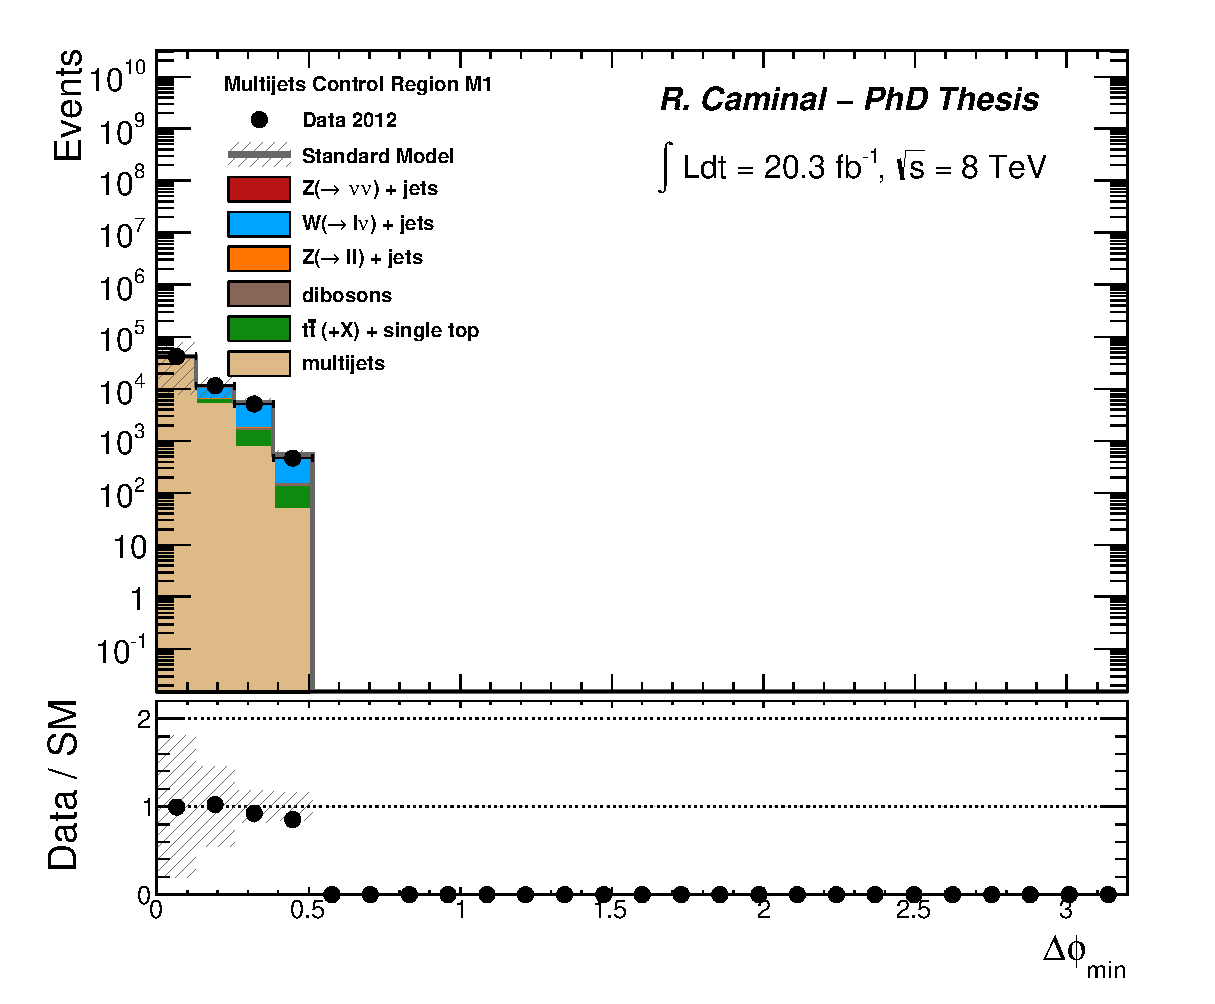
\includegraphics[width=0.495\textwidth]{Appendix_JetSmearingMethod/Figures/plot_Stop_A6_CRqcd_dPhi_min_fitted.eps}
      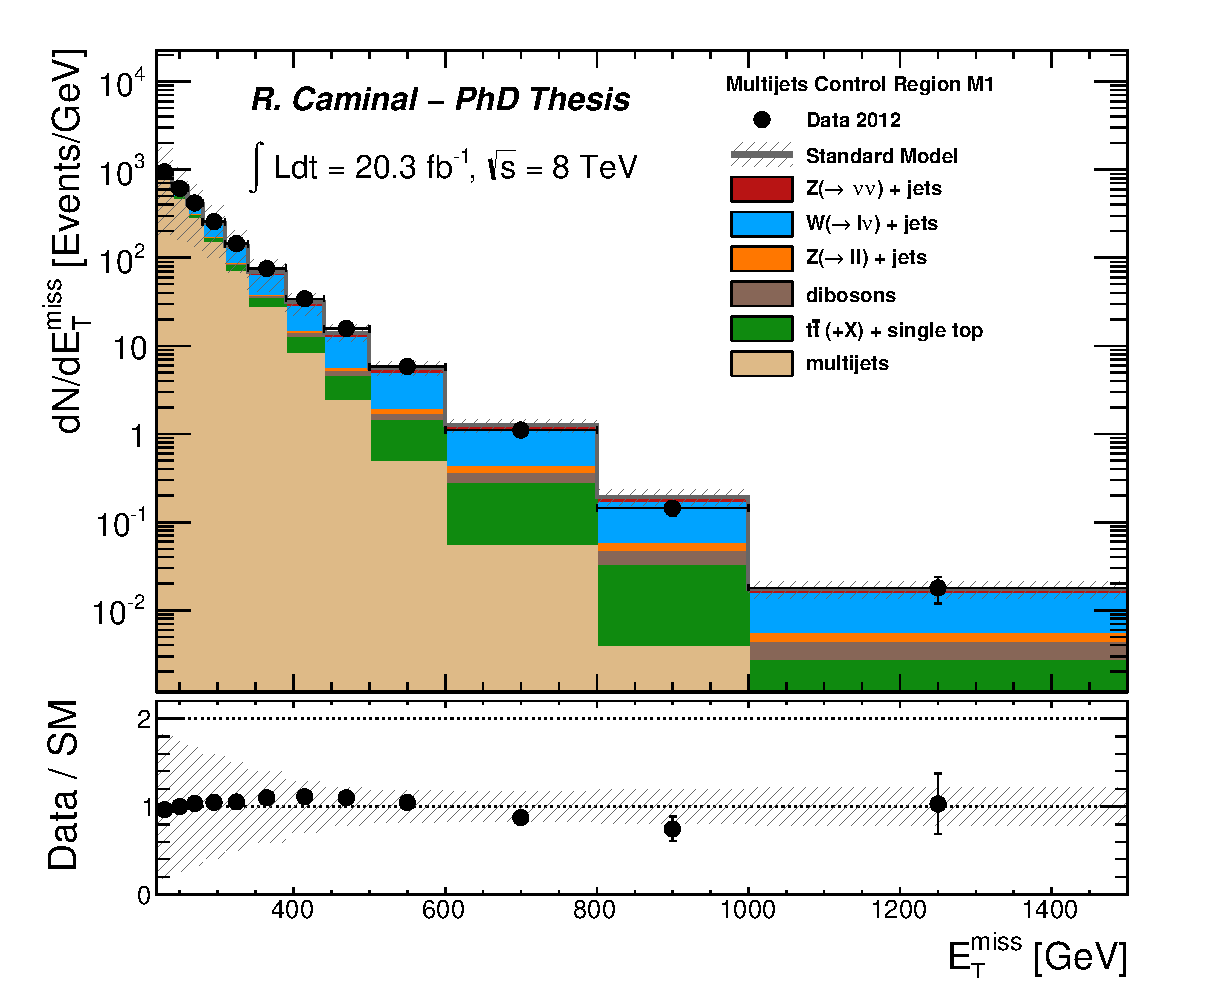
\includegraphics[width=0.495\textwidth]{Appendix_JetSmearingMethod/Figures/plot_Stop_A6_CRqcd_met_fitted.eps}
    }
    \mbox{
      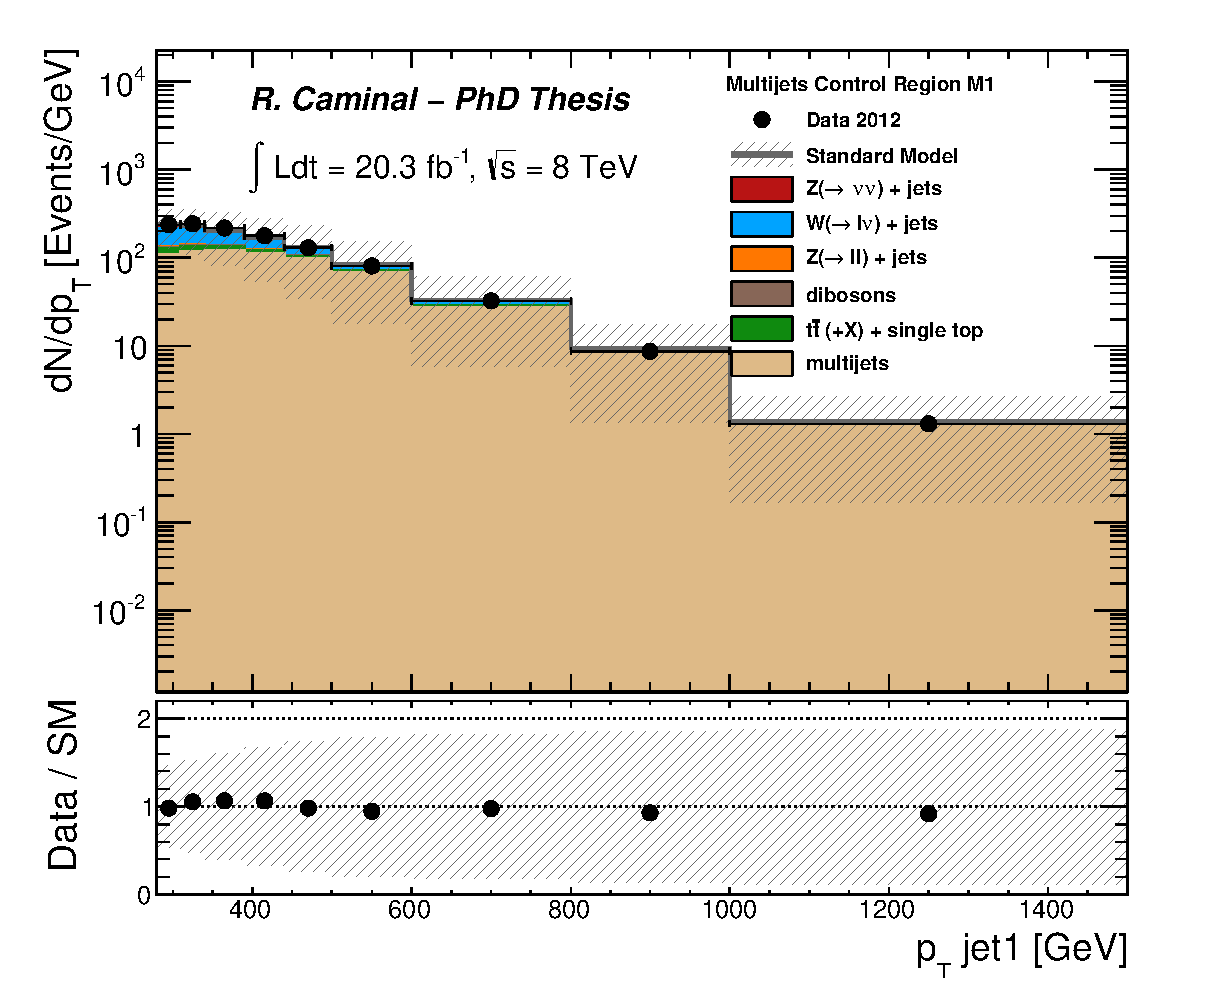
\includegraphics[width=0.495\textwidth]{Appendix_JetSmearingMethod/Figures/plot_Stop_A6_CRqcd_pt1_fitted.eps}
      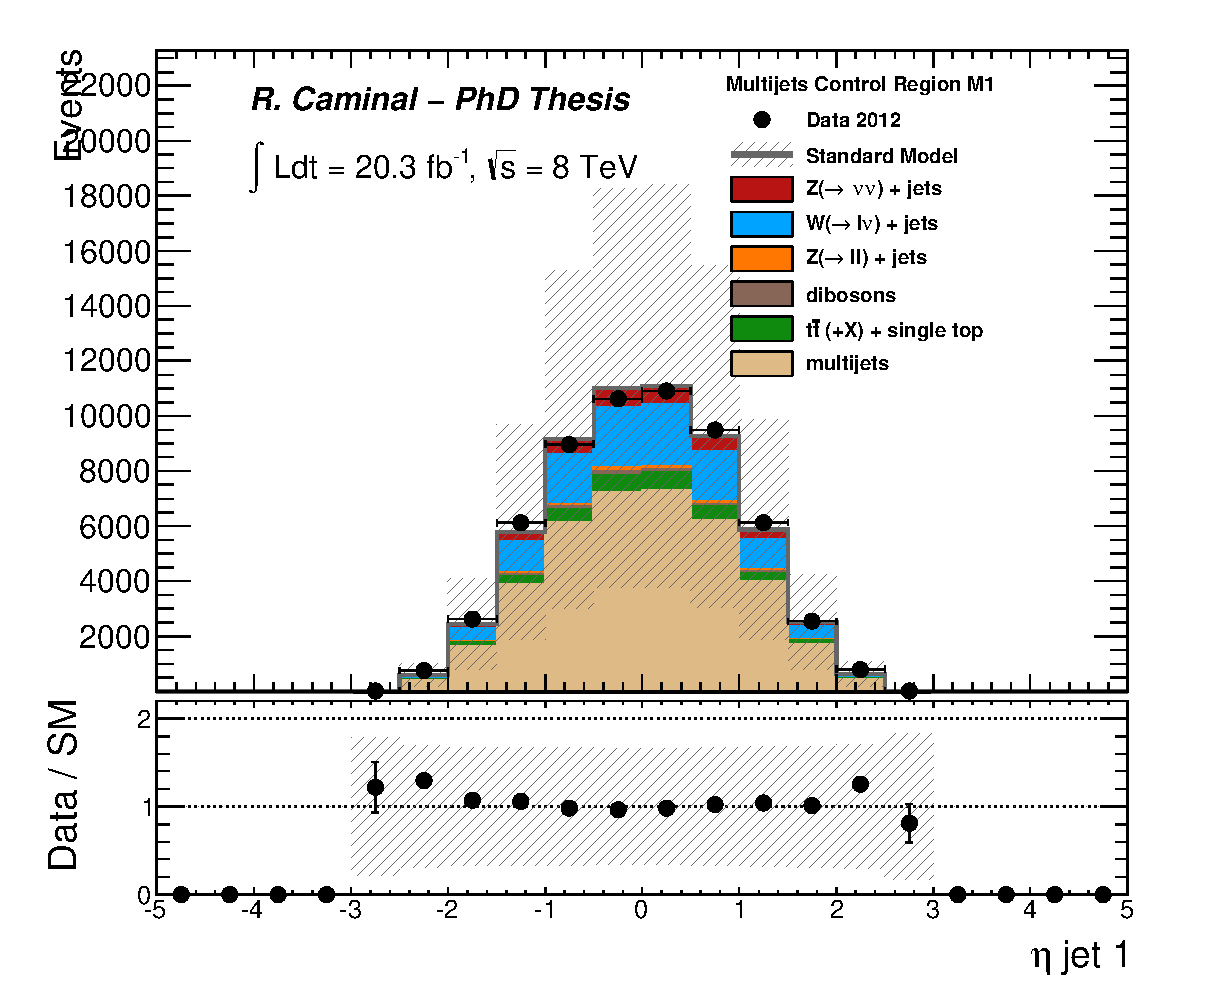
\includegraphics[width=0.495\textwidth]{Appendix_JetSmearingMethod/Figures/plot_Stop_A6_CRqcd_eta1_fitted.eps}
    }
    \mbox{
      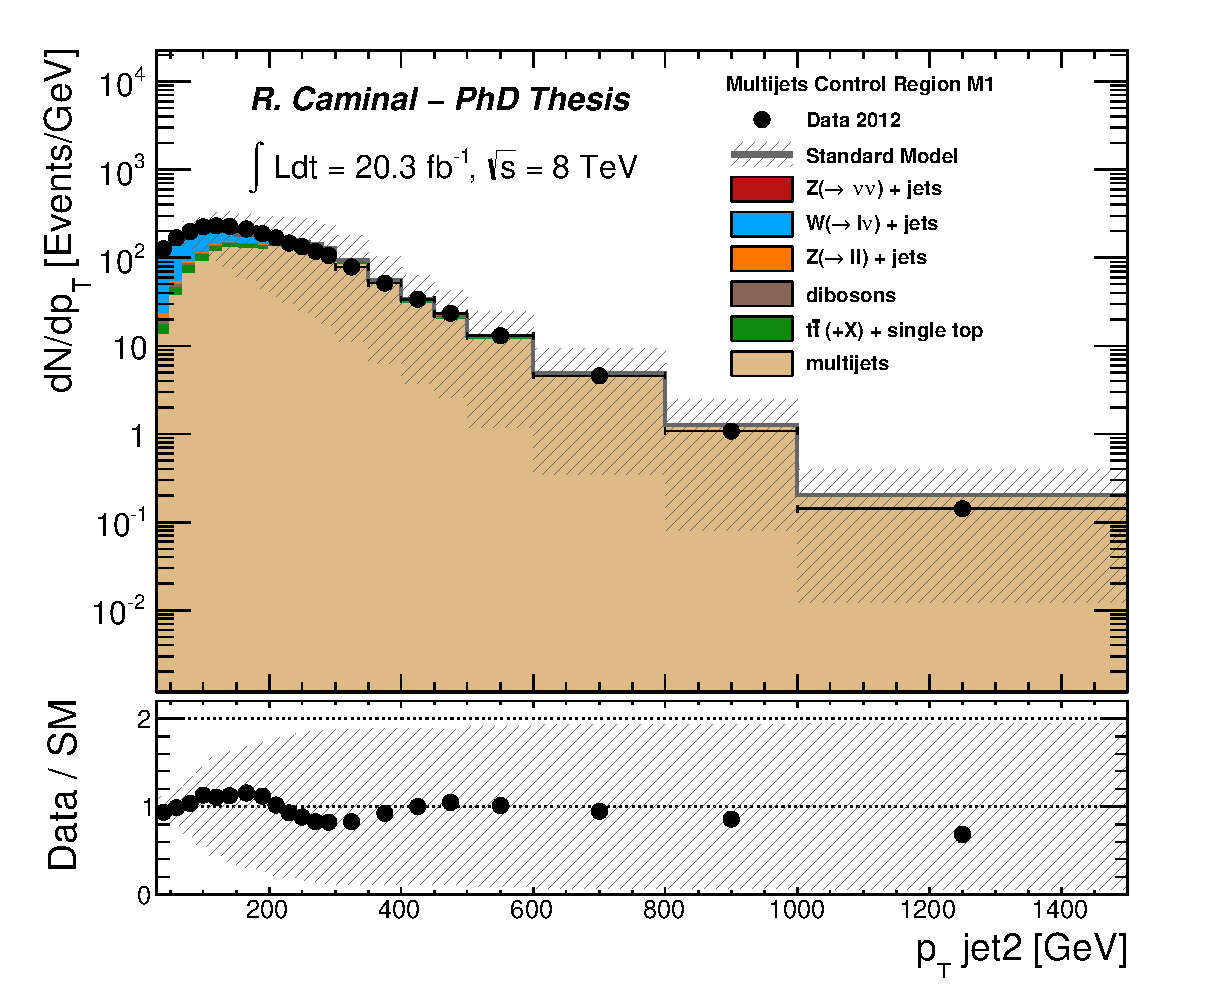
\includegraphics[width=0.495\textwidth]{Appendix_JetSmearingMethod/Figures/plot_Stop_A6_CRqcd_pt2_fitted.eps}
      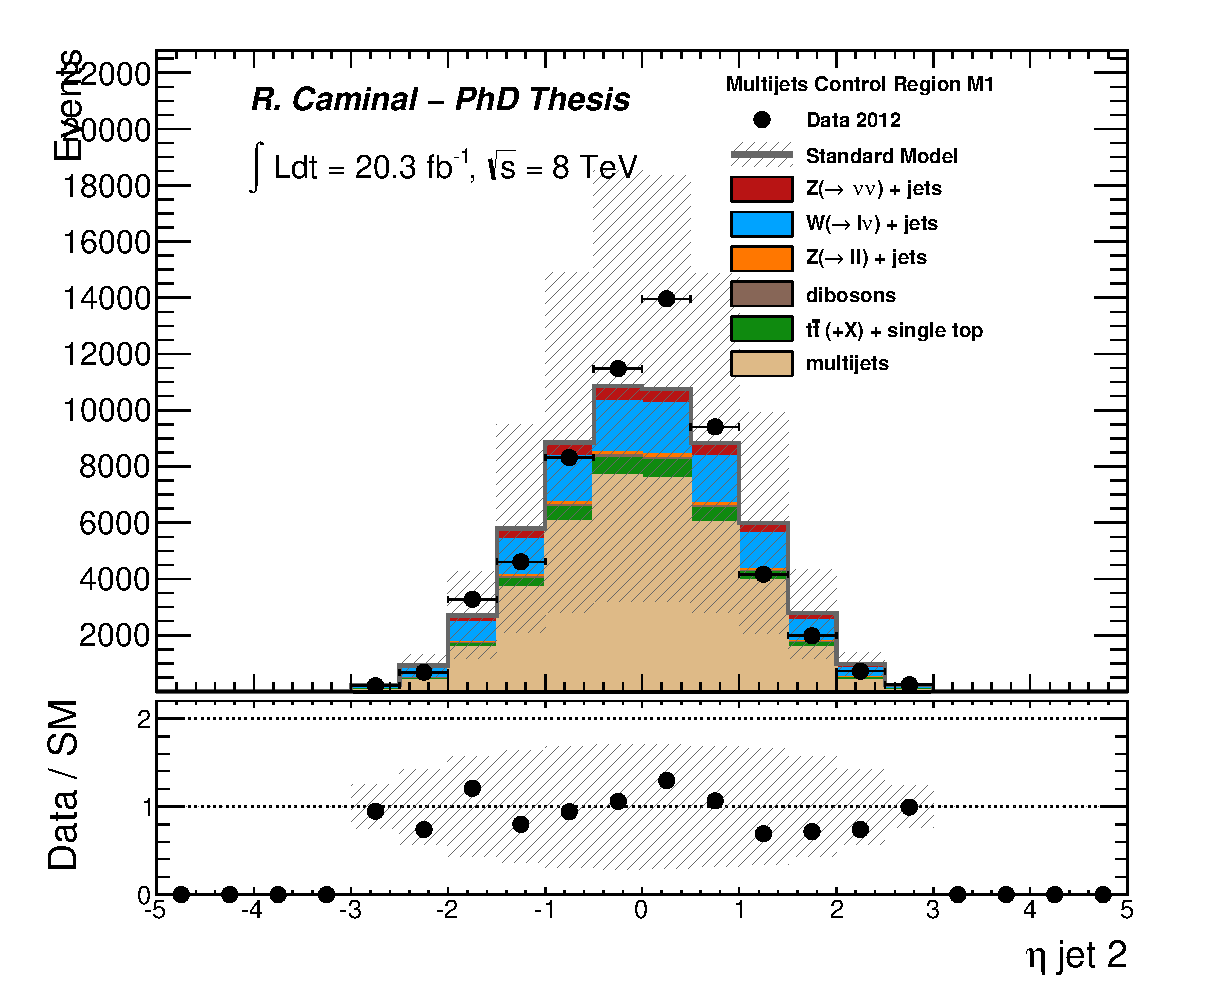
\includegraphics[width=0.495\textwidth]{Appendix_JetSmearingMethod/Figures/plot_Stop_A6_CRqcd_eta2_fitted.eps}
    }
  \end{center}
  \caption[Distributions of the minimum $\Delta\phi$ between the $\met$ and the leading jet $\pt$, the $\met$, the leading jet $\pt$ and $\eta$, and the second leading jet $\pt$ and $\eta$ for the multijet normalization region corresponding to the M1 selection cuts.]{Distributions of the minimum $\Delta\phi$ between the $\met$ and the leading jet $\pt$ (top left), the $\met$ (top right), the leading jet $\pt$ (middle left) and $\eta$ (middle right), and the second leading jet $\pt$ (bottom left) and $\eta$ (bottom right) for the multijet normalization region for the M1 selection cuts.}
  \label{fig:JetSmearingCheckPlots}
\end{figure}

